\section{Diodes: Basic Properties, and Clipper Circuits}
\label{lab_diodes}

%\makelabheader %(Space for student name, etc., defined in master.tex)

\bigskip

\begin{enumerate}[wide]

\item The circuit diagram below shows your transformer connected to two resistors, with the voltage across each resistor monitored by the oscilloscope.  (Both the primaries and secondaries are connected in parallel!)  Under the ``display'' menu of your scope, select a format of ``XY'' instead of the usual ``YT.''  Also, under the channel 2 menu, select ``invert on.'' In ``XY'' format, the scope will display a graph of channel 2 vs. channel 1, as opposed to showing them both vs. time as it usually does.  Since the two resistors in your circuit are identical, the display here should show a 45 degree diagonal line, the graph of $y = x$.  What does your display show if you disconnect either the channel 1 or channel 2 probe?
\vspace{-0.1in}
\begin{center}
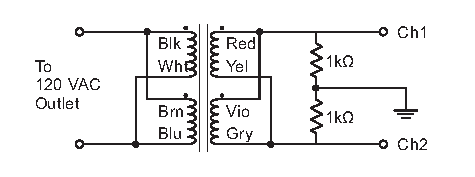
\includegraphics{diodes/diode_testing_circuit_1.eps}
\end{center}

\item If you replace the first resistor in your circuit with a diode, your oscilloscope shows you a graph of current vs. voltage for the diode.  Channel 1 (The X coordinate) is the voltage across the diode, and Channel 2 (The Y coordinate) is the voltage across the resistor, which is proportional to the current.  Use this to measure the IV curve of the following diodes: 1N4001, 1N4733, 1N4739, 1N34 (which may have no label, but is identifiable by two black lines), and each of your color LEDs.  What are their forward and reverse breakdown voltages, $V_F$ and  $V_R$?  What kind of diode is each of these?  (Silicon, Germanium, Zener....) \label{part_measuring_diode_iv} \label{part_diode_measurements}
\vspace{-0.1in}
\begin{center}
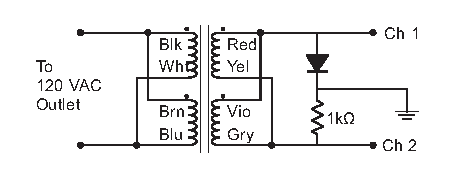
\includegraphics{diodes/diode_testing_circuit_2.eps}
\end{center}

\item You have now seen that when a diode is forward-biased (that is, when it has current going through it in the direction of the arrow) that the voltage drop $V_F$ across it is fairly constant, independent of current.  ($V_F \approx 0.7$ volts for a silicon diode, $V_F \approx 1.8$ volts for a red LED.)  To make your red LED light up, you want a current through it of about 10~mA; much more than that would blow it out.  But if you hook the LED directly to a known voltage source, the actual current through it is hard to control precisely.  Instead, you typically connect the LED to a power supply in series with a resistor, as shown below.  In the circuit below, what value of resistor would yield a current of 10~mA through the LED?  Test it out, and make changes if you don't measure 10~mA.  Also, what is the power dissipated in the resistor and in the diode?
\vspace{-0.1in}
\begin{center}
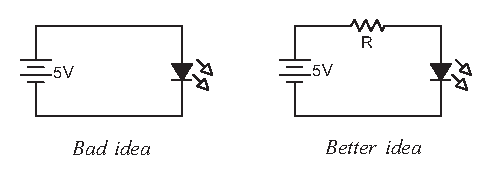
\includegraphics{diodes/led_with_resistor.eps}
\end{center}

\item Return your scope to ``YT'' mode, and \textit{do not forget to turn the Ch2 invert OFF}.  Build the ``series clipper'' circuit pictured below, using a 1N4001 diode and a load resistance of 100~k$\Omega$.  Make a sketch of the input waveform and the output waveform.  Make precise measurements of the peak positive and negative input voltages, and the peak positive and negative output voltages.  Are they exactly the same?  (You may want to shift the vertical positions of your traces and increase the scale on your scopes for more precise measurements.)  Also predict how your graph will change if you reverse the polarity of the diode, and test your prediction.
\begin{center}
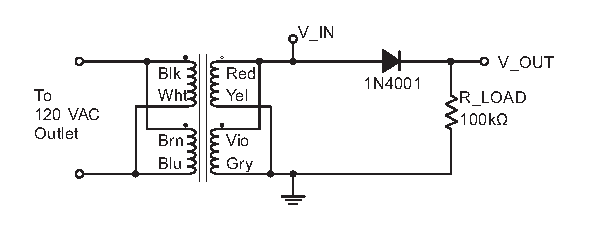
\includegraphics{diodes/series_clipper.eps}
\end{center}

\item Build the ``shunt clipper'' circuit picture below, using a 1N4001 diode.  Use a 1~k$\Omega$ resistor for $R_1$ and a load resistance of 100~k$\Omega$.  Again, make a sketch of the input waveform and output waveform, and carefully measure the peak positive and negative input and output voltages.  What is the maximum instantaneous current through the diode?  \label{part_shunt_clipper}
\begin{center}
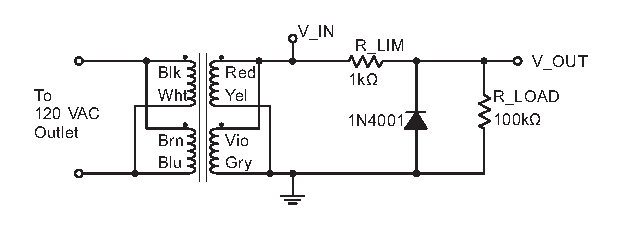
\includegraphics{diodes/shunt_clipper.eps}
\end{center} 
\item Think carefully about the role of $R_{LIM}$.  Your transformer has a very low output impedance of about 2~$\Omega$.  If the 1~k$\Omega$ resistor were removed from the circuit, it would be as if you set $R_{LIM} = 2$~$\Omega$.  In that case, what would be the maximum instantaneous current through the diode?  (Hint: consider both extremes, $V_{IN} = \pm V_{MAX}$.) What would be the maximum instantaneous power dissipated in the diode?  What would be the effect of all of that current and power on the diode?  The job of $R_{LIM}$ is to limit the power and current in the diode.

\item Predict how the output voltages of the ``series clipper'' and the ``shunt clipper'' would be affected if the load resistance $R_{LOAD}$  were changed to 1~k$\Omega$.  Check your predictions by building the circuits and testing them. What can you conclude about which design is better for producing high currents?  

%\pagebreak
\item The circuit below is called the ``biased shunt clipper.''  The diode's polarity has been reversed (just for variety), but more importantly it is now connected to a non-zero reference voltage instead of ground.  Build the circuit and sketch the resulting output waveform for $V_{OUT}$.  What is the relationship between $V_{OUT}$ and the voltage at the junction between $R_3$ and $R_4$?  Also, why is it necessary to use an op-amp in this circuit rather than connecting the diode to $R_3$ and $R_4$ directly?  If you did omit the op-amp, how would you have to adjust the values of your resistors?
\label{part_biased_shunt_clipper}
%\vspace{-0.1in}
\begin{center}
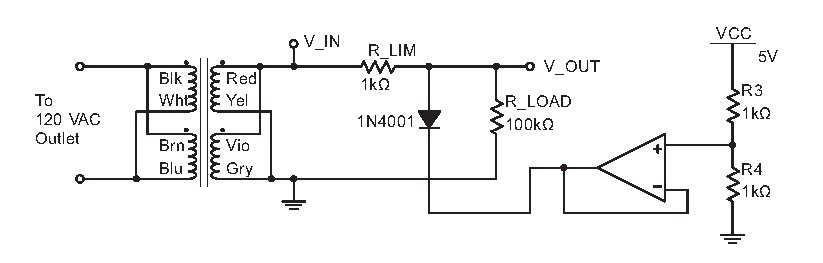
\includegraphics{diodes/biased_shunt_clipper2.eps}
\end{center} 
%\vspace{-0.1in}

\item Show how you could modify the biased shunt clipper above so that the output voltage never dips below 0.0 volts, as opposed to $-0.7$ volts for the unbiased shunt clipper you built in part~\ref{part_shunt_clipper}.   (Incidentally, there's a very slick way to guarantee exactly the voltage you need at the op-amp input $V_+$ without having to calclate precise resistor values.  Can you find it?)  \label{part_biased_clipper_zero}

\item Another way to build clippers that work at a variety of voltages is to use Zener diodes with specific values of $V_R$.  Predict the maximum and minimum output voltages of the circuit below, which uses a 1N4733 Zener diode.  Build the circuit, and test your predictions.  What is the maximum instantaneous power dissipated by the diode?  (Consider both $V_{Diode}=V_F$ and $V_{Diode}=V_R$.  \label{part_zener_shunt_clipper}
%\vspace{-0.1in}
\begin{center}
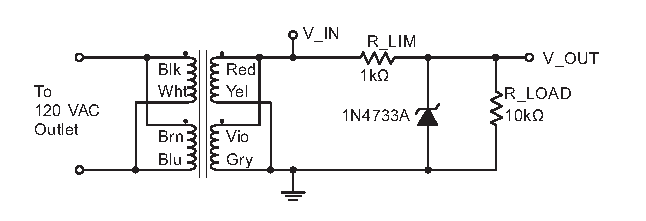
\includegraphics{diodes/zener_shunt_clipper.eps}
\end{center} 
%\vspace{-0.1in}
 
\item The circuit below uses two Zener diodes in series.  Again, predict the output of this circuit, then test your prediction.  How would you modify this circuit to make a shunt clipper that gives $V_{-PEAK} = -9.7$~V and $V_{+PEAK} = +5.7$~V.   (Hint: You don't need a biased clipper for this, because you can replace the 1N4733 with any kind of diode you want.  In fact, if you look back at your measurements from part~\ref{part_diode_measurements}, you'll find one diode that's just \textit{perfect} for what you need to do here.)  
%\vspace{-0.1in}
\begin{center}
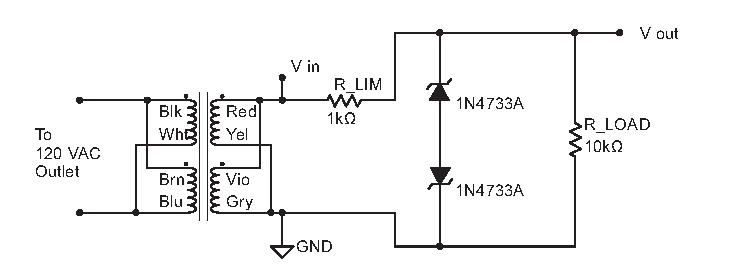
\includegraphics{diodes/double_zener_shunt_clipper.eps}
\end{center} 
 
\end{enumerate}



\textbf{Possible Exam Questions:}

\begin{itemize}

\item For the circuit drawn in part~\ref{part_biased_shunt_clipper}, calculate the maximum instantaneous current in the diode.

\item Draw a graph of current vs. voltage for (a) a yellow LED, (b) a germanium diode, and (c) a Zener diode, including both positive and negative voltages.

\item Design a biased shunt clipper that limits the output voltage to a maximum of 4.5 volts, regardless of the input voltage.

\item For the circuit drawn in part~\ref{part_zener_shunt_clipper}, calculate the maximum instantaneous power dissipated in the resistor $R_{LIM}$. 

\item What are the relative advantages and disadvantages of a series clipper vs. a  shunt clipper?

\item As with all previous labs, you should be able to recreate any circuit in this lab from memory, choosing appropriate values of components as needed to get any desired behavior.  You should also be able to calculate the value of voltage or current for any component given a diagram of any circuit you built here.

\item In Lab~\ref{lab_op-amps} part~\ref{part_proportional_controller} you built a proportional controller, where the output voltage was proportional to the difference between a setpoint temperature and a measured temperature.  The idea was that the output voltage could go to a heater, which would heat just enough to maintain a constant temperature on something like a hotplate.  But if you think about it, there was one small problem: the heater would also receive current (albeit negative) if the measured temperature was \textit{higher} than the setpoint, which would make the hotplate heat up even more!  Show how you could integrate the clipper circuit you built in part~\ref{part_biased_clipper_zero} of this lab into your circuit from Lab~\ref{lab_op-amps} part~\ref{part_proportional_controller} to prevent this problem.


\end{itemize}






